\documentclass[11pt]{article}
\usepackage[utf8]{inputenc}
\usepackage[labelfont=bf]{caption}
\usepackage[compact]{titlesec}
\usepackage{appendix}
\usepackage{graphicx,amsmath,booktabs,subcaption,placeins,mathtools,multirow} % All of the classics
\usepackage{tikz}
\usepackage[activate={true,nocompatibility},
    final,
    tracking=true,
    kerning=true,
    spacing=true,
    factor=1100,
    stretch=10,
    shrink=10]{microtype}
    \microtypecontext{spacing=nonfrench}
\usepackage[colorlinks,
    linkcolor=teal,
    citecolor=teal,
    filecolor=teal,
    urlcolor=teal]{hyperref}
\usepackage[margin=1in]{geometry} % 1in margins
\usepackage[version=4]{mhchem}

% -- Use the Charter fonts as base fonts, fixup math-mode display
\usepackage[charter]{mathdesign}
\usepackage[scaled=.96,osf]{XCharter}
\linespread{1.04}
\usepackage[backend=biber,style=nature,backref=true]{biblatex} %author-year for in-text content
%\hyphenpenalty=750
\usepackage{cleveref}
%-------------------end standard preamble-------------------------
\newcommand{\units}[2]{\frac{\text{#1}}{\text{#2}}\,}
\newcommand{\unit}[1]{\; \text{#1}\,}

\titlespacing{\section}{0pt}{2ex}{1ex}
\titlespacing{\subsection}{0pt}{1ex}{0ex}

\title{TANGLES: modeling supercoiling-dependent feedback}
\author{Christopher Johnstone}
\date{}

\addbibresource{main_library.bib}

\begin{document}
\maketitle

\section{Introduction}
Mammalian genomes are enormously complex systems regulated over a vast range of length and time scales; ongoing transcription-linked processes constantly reshape chromatin, cell division and the associated genomic replication regularly disrupt the structure of the genome \parencite{johnstoneUnderstandingEngineeringChromatin2020}. Extensive work in the fields of synthetic and systems biology has demonstrated the wide applicability of concentration-mediated regulation, including native and synthetic DNA-binding proteins (including zinc-finger proteins, dCas9 fusions, and transcription factors), small molecule aptamers, and miRNA regulators.
A rich modeling framework based on the predictions of ordinary differential equation models and discrete stochastic simulation models well predicts the behavior of these systems.
Some recent notable forays into novel regulatory methods include systems that maintain and creates synthetic epigenetic memory \parencite{parkEngineeringEpigeneticRegulation2019} and the mechanical regulation imparted by synthetic liquid-liquid phase condensates \parencite{shinLiquidNuclearCondensates2018}.

Recently, synthetic circuits have been designed to take advantage of the rich transcription-chromatin feedback network underlying native gene regulation. Mimicking the proximity-dependent behavior of native systems, synthetic enhancer-promoter circuits have been designed in \textit{Drosophila} that depend on the presence of a local contact domain \parencite{yokoshiVisualizingRoleBoundary2020}. Deleting one of the contact domain boundaries decreased reporter output without significantly perturbing gene expression in adjacent contact domains \parencite{yokoshiVisualizingRoleBoundary2020}.
In mammalian cells, insertion and deletion of CTCF-binding sites changes the activity of nearby promoters by modifying intra-domain enhancer-promoter contacts \parencite{jiaTandemCTCFSites2020}. Combining this work with recent programmable recombinases and flipases may allow for live-cell controllable contact domain engineering \parencite{guoCRISPRInversionCTCF2015,weinbergHighperformanceChemicalLightinducible2019}.

One key regulatory strategy that may be important in native circuits but is hitherto underutilized in synthetic circuits is supercoiling-mediated feedback---a mechanism dependent on the under- and over-winding of DNA caused by the activity of RNA polymerases and other enzymes. Such a feedback mechanism would be affected by changes in chromatin syntax, including the placement, orientation, and composition of circuit elements.
In order to create synthetic circuits capable of utilizing biophysical feedback, the physical mechanisms by which transcription induces feedback must be understood. To understand these biophysical mechanisms, we require a chromatin model that includes the process of transcription. Many constraint-based models have successfully predicted chromatin structures from experimental contact domain information (Hi-C maps) \parencite{distefanoTranscriptionalActivationCell2020,serraRestraintbasedThreedimensionalModeling2015,abbasIntegratingHiCFISH2019}. These models coarse-grain chromatin as a self-interacting 3D polymer, but do not explicitly represent transcription---a key process we want to model. Phenomenological models, which model polymerase binding using a supercoiling-dependent energy term calibrated from experiments but do not simulate polymerase motion, have been successful in modeling the effects of supercoiling for bacterial gene expression  \parencite{elhoudaiguiBacterialGenomeArchitecture2019a,yeungBiophysicalConstraintsArising2017}. An intermediate method for modeling the effects of supercoiling is to abstract details of the helical polymer model into a statistical mechanics model that predicts energy and torque responses arising from perturbations such as transcription. Such a model has been developed by \textcite{markoSupercoiledBraidedDNA1997,markoTorqueDynamicsLinking2007} and \textcite{sevierPropertiesGeneExpression2018}. Such an intermediate model allows us to understand how the physical motion of polymerases leads to feedback, without having to do detailed molecular simulation \parencite{fosadoNonequilibriumDynamicsAction2021}.

Here, we present an extension of the model first proposed in \parencite{sevierMechanicalPropertiesDNA2019}. By modeling the joint effect of supercoiling-dependent polymerase initiation and polymerase stalling, we predict a wide range of emergent feedback behaviors, that may be used to both inform novel synthetic circuit designs and explain observed native phenomena.

\section{Model}
Simulating the behavior of native and synthetic circuits under the influence of transcription-induced feedback requires an model that integrates explicitly-modeled polymerase motion and RNA- and protein-mediated feedback mechanisms.
Our method combines three modeling levels: an ordinary differential equation model that simulates the continuous progression of polymerases loaded onto DNA, a core stochastic model that models supercoiling-dependent polymerase initiation, and a user-specified stochastic layer that allows for simulation of other regulatory interactions such as promoter activity dependent on protein production and degradation.

Following previous work, modeled the motion of polymerases using an ODE model where each polymerase is defined by three variables---the (one-dimensional) position of the polymerase along the DNA \(z_i\), the length of the single-stranded nascent RNA \(x_i\), and the excess twist relative to relaxed DNA at the location of the polymerase \(\phi_i\) \parencite{markoTorqueDynamicsLinking2007,sevierPropertiesGeneExpression2018}.

By storing the excess twist of DNA, we can easily calculate. On the rele
On the relevant length scale of synthetic circuits (O(10-100kb)),

\section{Results}

\begin{figure}[h]
    \centering
    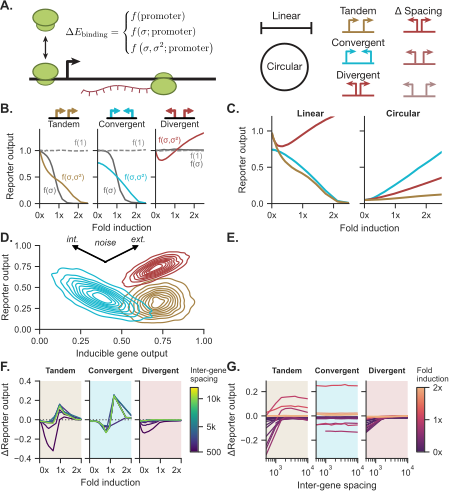
\includegraphics{figures/modeling_paper/fig_1.pdf}
    \caption{}
\end{figure}
\begin{figure}[h]
    \centering
    \includegraphics{figures/modeling_paper/fig_2.pdf}
    \caption{}
\end{figure}
\begin{figure}[h]
    \centering
    \includegraphics{figures/modeling_paper/fig_4.pdf}
    \caption{}
\end{figure}

\section{Discussion}

Supercoiling density is defined:
\begin{equation}
    \sigma = \frac{\phi_i - \phi_{i - 1}}{\omega_0 | z_{i} - z_{i-1}|}
    \label{eq:sc_density}
\end{equation}
where \(\phi\) defines a \emph{linking number constraint}. While this term is most easily identified with the local DNA excess twist, it is truly a linking number constraint that takes into account both twist and writhe. The asymmetry between these two forms is accounted for in the phase transition in the underlying statistical mechanical model.

Based on a statistical-mechanics model that calculates the torque as a function of supercoiling density:
\begin{equation}
    \tau(\sigma) = \begin{dcases} \tau_S \sigma & |\sigma| < |\sigma_s| \\ \tau_0 \text{sgn}(\sigma) & |\sigma_s| \leq |\sigma | \leq |\sigma_p| \\ \tau_P \sigma & |\sigma_p| \leq |\sigma|\end{dcases}
\end{equation}



\section{Claims}

\subsection{ DNA supercoiling dynamics confer rapid, tunable coupling between adjacent genes in linear and circular contexts }
\begin{itemize}
    \item Supercoiling allows for regulation on timescales otherwise inaccessible by synthetic systems.

    \item (probably we should say something about noise and controlling for it via syntax)

    \item Divergent gene orientation can lead to strongly correlated bursting on short timescales.

    \item Supercoiling-dependent initiation, modeled here as an expansion based on assumptions reasonable for real systems, is a key supercoiling-dependent mechanism that is balanced against polymerase stalling.

    \item Expression context provides different boundary conditions, inducing different levels of supercoiling-dependent feedback.

    \item Regulatory systems involving supercoiling are capable of sense changes in genomic context, such as changes in adjacent gene expression and accessibility.
\end{itemize}


\clearpage
\subsection{Supercoiling-dependent intergene coupling supports rapid  transcriptional feedback, generating emergent patterns of expression}
\begin{itemize}
    \item The syntax of compact, simple gene cassettes provides a design parameter for specifying and tuning transcriptional feedback.

    \item Asymmetric polymerase initiation with respect to supercoiling density leads to physically-realistic asymptotic behavior.
\end{itemize}

\clearpage
\subsection{ Optimized circuit syntax supports enhanced toggle switch stability via DNA supercoiling }
\begin{itemize}
\item Supercoiling-dependent feedback can enhance the ultrasensitive response of synthetic regulatory motifs (toggle switch stability).
\end{itemize}

\clearpage
\subsection{DNA supercoiling provides a mechanism to tightly coordinate expression of proximal segmentation genes }
\begin{itemize}
    \item Supercoiling dependent initiation may underpin the stability of the \textit{her1},\textit{her7} clock circuit.

\end{itemize}

\subsection{Designing gene circuits to detect topoisomerase activity}
\begin{itemize}

    \item Cells transiting fate transitions show varying cell cycle rates and topoisomerase activity patterns, which are detectable via supercoiling-dependent feedback.
\end{itemize}

Through colocalization, native circuits appear to incorporate transcription-linked feedback mechanisms to both reduce noise and tune cell-state specific output in tightly regulated processes such as development. For example, in zebrafish, proper somite segmentation requires precise coordination of two clock genes, \textit{her1} and \textit{her7}. In addition to an auto-feedback loop, \textit{her1} and \textit{her7} are placed in a divergent syntax, with only 12-kb separating their coding regions. In engineered zebrafish where \textit{her1} and \textit{her7} are expressed from different chromosomes, irregular somites form as a result of reduced coordination of gene expression \parencite{zinaniPairingSegmentationClock2020}. Only through a combination of protein-mediated regulation and biophysical regulation does proper somite segmentation occur. In mammals as well, colocalization of regulatory elements may be necessary for proper development. For example, in mice, the \textit{Pitx1} gene is a regulator of hindlimb development. \textit{Pitx1} is in turn regulated by the \textit{Pen} enhancer, which is actively transcribed in both the forelimbs and hindlimbs. In wild-type mice, a contact domain encloses \textit{Pen} and \textit{Pitx1} only in the hindlimb; if this  \textasciitilde{}100kb genomic region is inverted to mimic the colocalization found in the hindlimbs, \textit{Pitx1} is ectopically expressed in the forelimbs \parencite{kragesteenDynamic3DChromatin2018}.

\section{Methods}
\subsection{ODE and stochastic simulation}
The core ordinary differential equations were simulated using a Tsitouras's explicit Runge-Kutte 4-5 order method \parencite{tsitourasRungeKuttaPairs2011}.
\parencite{rackauckasDifferentialEquationsJlPerformant2017}.

\subsection{Code availability}
Full simulation and figure-generating code is available at \url{https://github.com/GallowayLabMIT/tangles_model}.

\subsection{Acknowledgements}
The authors acknowledge the MIT SuperCloud and Lincoln Laboratory Supercomputing Center \parencite{reutherInteractiveSupercomputing402018} for providing HPC resources that have contributed to the research results reported within this paper.

\printbibliography

\clearpage
\appendix
\renewcommand{\appendixpagename}{Supplemental information}
\appendixpage
\section{Model design, derivation, and extension}
\label{sec:appendix:model}
The original transcription-supercoiling paper, \cite{sevierPropertiesGeneExpression2018}, relies on prior papers for relevant equation definitions needed to actually implement the model. The following work gathers all of these relevant equations and simulation constants together, then discusses my model extensions.

\subsection{Supercoiling model}
Why do we care about supercoiling at all? As noted in \textcite{markoTorqueDynamicsLinking2007}, at \(T = 300 \unit{K}\), \(k_b T = 4.1 \unit{pN nm}\), showing that
important mechanical properties are on the energy scale of \(k_b T\). Many of the later quantities we will solve for will have magnitude around 10-100 pN nm.

Supercoiling density is defined:
\begin{equation}
    \sigma = \frac{\phi_i - \phi_{i - 1}}{\omega_0 | z_{i} - z_{i-1}|}
    \label{eq:sc_density}
\end{equation}
where \(\phi\) defines a \emph{linking number constraint}. While this term is most easily identified with the local DNA excess twist, it is truly a linking number constraint that takes into account both twist and writhe. The asymmetry between these two forms is accounted for in the phase transition in the underlying statistical mechanical model.

Based on a statistical-mechanics model that calculates the torque as a function of supercoiling density:
\begin{equation}
    \tau(\sigma) = \begin{dcases} \tau_S \sigma & |\sigma| < |\sigma_s| \\ \tau_0 \text{sgn}(\sigma) & |\sigma_s| \leq |\sigma | \leq |\sigma_p| \\ \tau_P \sigma & |\sigma_p| \leq |\sigma|\end{dcases}
\end{equation}

what???
By expanding the free energy as a power series in \(\sigma\), we get the symmetric form:
\begin{equation}
    S = \begin{dcases}
        -g + \frac{1}{2} c_s \sigma^2 & |\sigma| < |\sigma_s| \\
        \frac{-g}{1 - \frac{p}{c_s}} + \sqrt{\frac{2 p g}{1 - \frac{p}{c_s}}} |\sigma| & |\sigma_s| < |\sigma| < |\sigma_p| \\
        \frac{1}{2} p \sigma^2 & |\sigma| > |\sigma_p|
    \end{dcases}
\end{equation}

where the following quantities are defined:
\[\tau_S = \frac{c_s}{\omega_0} \qquad \tau_0 = \sqrt{\frac{2 pg}{\omega_0^2 \left(1 - \frac{p}{c_s}\right)}} \qquad \tau_P = \frac{p}{\omega_0} \]
\[|\sigma_s| = \frac{1}{c_s} \sqrt{\frac{2pg}{1 - \frac{p}{c_s}}} \qquad |\sigma_p| = \frac{1}{p} \sqrt{\frac{2pg}{1 - \frac{p}{c_s}}}\]
\[g = f - \sqrt{\frac{k_B T f}{A}} \qquad c_s = c \left[1 - \frac{C}{4A} \sqrt{\frac{k_B T}{A f}}\right]\]


While the cubic term can also be calculated and accounts for asymmetry between under- and over-winding, \textcite{markoTorqueDynamicsLinking2007} argues that this effect is small for realistic physiological conditions.


Summarizing, once we specify \(p, g, c_s, \omega_0\), we have a model for the torque of our system.

In these equations, we rescale
the bend persistence length \(A\), the twist persistence length of stretched DNA \(C\), and the twist persistence length of the plectonemic
state \(P\). Because plectonemes reduce twist into writhe, we expect \(P < C\).
\[c = k_B T C \omega_0^2 \qquad p = k_B T P \omega_0^2\]

\begin{table}[h]
    \centering
    \begin{tabular}{@{}lll@{}}
        \toprule
        Variable & Value & Reference \\
        \midrule
        \(k_b\) & \(0.01381 \units{pN nm}{K}\) & - \\
        \midrule
        A & \(50\)nm & \parencite{markoTorqueDynamicsLinking2007} \\
        C & \(95 \pm 10\)nm & \parencite{markoTorqueDynamicsLinking2007} \\
        P & \(24 \pm 3\)nm & \parencite{markoTorqueDynamicsLinking2007} \\
        \(\omega_0\) & 1.85 \(\units{1}{nm}\) & \parencite{sevierPropertiesGeneExpression2018}, others \\
        \bottomrule
    \end{tabular}
    \caption{Key values}
    \label{tab:constants}
\end{table}


\subsection{Dynamic model}
Following \textcite{sevierPropertiesGeneExpression2018}, we define an identical dynamics model for modeling the motion of polymerases over the DNA.

Briefly, for each polymerase, this model tracks the position \(z_i\), transcript length \(x_i\), and excess DNA twist \(\phi_i\) of each RNAP. We create a \emph{linking number constraint (LNC)} by specifying \(\phi\) at any genomic location, which means that each RNAP sets an LNC. We use dynamic equations to model the motion of RNAP against either fixed or free boundary conditions.

As mentioned in the main text, the dynamic equations are:

\begin{equation}
    \omega_0 \frac{d z_i}{dt} = \frac{d \theta_i}{dt} + \frac{d \phi_i}{dt} \qquad \qquad \tau(z_i, \phi_{i-1}, \phi_{i+1}) = \eta x_i^n \frac{d\theta_i}{dt} - \chi \frac{d\phi_i}{dt}
\end{equation}

By solving the left equation for \(\frac{d \theta_i}{dt}\) and substituting it into the right equation, we get:
\[\tau(z_i, \phi_{i-1}, \phi_{i+1}) = \omega_0 \frac{dz_i}{dt} \eta x_i^n - \eta x_i^n \frac{d\phi_i}{dt} - \chi \frac{d\phi_i}{dt}\]
Solving for \(\frac{d\phi_i}{dt}\), we get a dynamic equation for the differential linking number constraint:

\begin{equation}
    \frac{d\phi_i}{dt} = \omega_0 \frac{dz_i}{dt} \frac{\eta x_i^n}{\chi + \eta x_i^n} - \frac{\tau(z_i, \phi_{i-1}, \phi_{i+1})}{\chi + \eta x_i^n}
\end{equation} \label{eq:phi_deriv}

To model polymerase stalling, instead of using Sevier's function, we use a parameterized function that explicitly depends on a stall torque and a torque width \(\Delta \tau\) over which stalling begins to occur:
\begin{equation}
    \frac{dz_i}{dt} = \frac{v_0}{1 + \exp\left(\frac{|\tau(z_i, \phi_{i-1}, \phi_{i+1}) - \tau_s|}{\Delta \tau_s}\right)}
\end{equation} \label{eq:velocity}

Equations \ref{eq:phi_deriv} and \ref{eq:velocity} along with the simple \(\frac{dx_i}{dt} = \frac{dz_i}{dt}\) together represent a complete coupled set of ODEs that can be simulated, as long as the following constants are defined:

\begin{table}[h]
    \centering
    \begin{tabular}{@{}lll@{}}
        \toprule
        Variable & Value & Reference \\
        \midrule
        \(\chi\), DNA twist mobility  & \(0.01381 \unit{s pN nm}\) & \parencite{sevierPropertiesGeneExpression2018} \\
        \(\eta\), mRNA drag coefficent  & \(1/20 \unit{pN}\) & \parencite{sevierPropertiesGeneExpression2018} \\
        \(n\), Drag scaling exponent  & \(1\) & \parencite{sevierPropertiesGeneExpression2018} \\
        \(v_0\), Maximum polymerase velocity  & \(20 \units{nm}{s}\) & \parencite{sevierPropertiesGeneExpression2018} \\
        \(\tau_s\), Polymerase stall torque  & \(12 \unit{pN nm}\) & \parencite{sevierPropertiesGeneExpression2018} \\
        \(\Delta \tau_s\), Polymerase stall width  & \(3 \unit{pN nm}\) & This proposal \\
        \(\delta\), Polymerase radius  & \(15 \unit{nm}\) & \parencite{sevierPropertiesGeneExpression2018} \\
        \bottomrule
    \end{tabular}
    \caption{Key dynamic model values}
    \label{tab:dynamic_model_constants}
\end{table}

\subsection{Polymerase readthrough}
To model polymerase readthrough, I extended the model implementation to allow for polymerases to move for either a period of time or a certain distance after reaching the simulated PAS site. Readthrough times/distances were pulled from an exponential waiting time distribution.

\subsection{Supercoiling-dependent initiation}
I extended the Sevier and Marko model to account for supercoiling-dependent initation, starting with developing desired model properties based on literature observations. The rest of this appendix details this process, in addition to the initial model formulation and useful simplifications.

\subsubsection{Literature observations}
A naked DNA bead experiment (\textcite{revyakinPromoterUnwindingPromoter2004}) found that positive and negative supercoiling affected RNAP polymerase binding rates. When a polymerase bound, approximately 1.2 turns of DNA unwound (13 base pairs, or 4.42nm). This level of unwinding agrees with crystal structures of the bacterial T7 RNAP bound to DNA, as in Figure \ref{fig:rnap_bound}.

\begin{figure}[h]
    \centering
    %\includegraphics[width=.5\linewidth]{figures/1MSW}
    \caption{Crystal structure (PDB: 1MSW) of T7 RNAP bound to DNA. The protein is shown in brown, with the template DNA strands in green and olive.
             A 13 base pair region that is actively being read is fully melted.}
    \label{fig:rnap_bound}
\end{figure}

This bead study found that for a typical bacterial promoter, RNAP binding occurred reversibly. The mean time between RNAP binding events was measured and related to a kinetic model. The mean time between binding events can be related to a promoter-on rate. Once the DNA torque reached the constant-torque regime, the promoter-on rate became constant.

\subsubsection{Modeling goals}
Based on the literature observations, some desired properties of a model would be:
\begin{itemize}
    \item In the constant-torque supercoiling regime, the RNAP on rate remains constant, as in \textcite{revyakinPromoterUnwindingPromoter2004}.
    \item Negative supercoiling promotes RNAP binding, whereas negative supercoiling inhibits RNAP binding.
    \item The promoter on rate depends just on the local supercoiling density and the nearest LNCs, not on the position of the promoter relative to the bounding LNCs.
    \item Plotted as a function of supercoiling density (from \(\sigma = -.1\) to \(\sigma = .1\)), the response is roughly sigmodial, to match phenomenological models (such as \textcite{elhoudaiguiBacterialGenomeArchitecture2019a}).
\end{itemize}

However, the first and fourth goals are contradictory; if the RNAP on-rate remains constant, then we won't get a sigmodial shape when plotted versus supercoiling density.

\FloatBarrier
\subsubsection{Dual-LNC model}
To model this unwinding, we add two new LNCs, spaced 13 base pairs apart. To start, all of these have specific linear locations \(z\) and rotations \(\phi\), but we will show that under some relatively valid assumptions, the specific location of the new LNCs does not matter.

\begin{figure}[h]
    \centering
    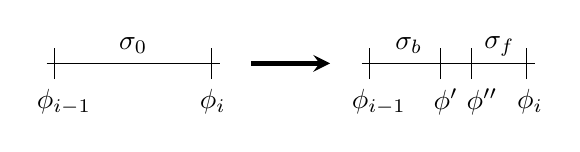
\begin{tikzpicture}
        \draw (-5.1, 0) -- (-2.9, 0);
        \draw (-5, -.2) -- (-5, .2);
        \draw (-3, -.2) -- (-3, .2);
        \node [below] at (-4.88, -.2) {$\phi_{i-1}$};
        \node [below] at (-2.99, -.2) {$\phi_i$};
        \node [above] at (-4, 0) {$\sigma_0$};

        \draw [ultra thick,->,>=stealth] (-2.5, 0) -- (-1.5, 0);

        \draw (-1.1, 0) -- (1.1, 0);
        \draw (-1, -.2) -- (-1, .2);
        \draw (1, -.2) -- (1, .2);
        \draw (.3, -.2) -- (.3, .2);
        \draw (-.1, -.2) -- (-.1, .2);
        \node [below] at (-.88, -.2) {$\phi_{i-1}$};
        \node [below] at (1.04, -.2) {$\phi_i$};
        \node [below] at (.43, -.2) {$\phi''$};
        \node [below] at (-.03, -.2) {$\phi'$};
        \node [above] at (.65, -.04) {$\sigma_f$};
        \node [above] at (-.5, 0) {$\sigma_b$};
    \end{tikzpicture}
    \caption{Diagram of the addition of two LNCs}
    \label{fig:lnc_diagram}
\end{figure}

We then put an angular restriction on the two new linking number constraints. By subtracting off the excess angle \(\phi\) that the undisturbed DNA has prior to RNAP binding (linearly interpolated because we assume complete supercoiling relaxing), we can define:
\begin{equation}
    \Delta \phi' = \phi' - \left(\phi_{i - 1} + \frac{z' - z_{i-1}}{z_i - z_{i-1}} (\phi_i - \phi_{i-1})\right)
\end{equation}

\begin{equation}
    \Delta \phi'' = \phi'' - \left(\phi_{i - 1} + \frac{z'' - z_{i-1}}{z_i - z_{i-1}} (\phi_i - \phi_{i-1})\right)
\end{equation}

For unwinding of the region bound to the RNAP to occur, we impose two constraints:
\begin{equation}
    |\Delta \phi'| + |\Delta \phi''| = 1.2 \cdot 2 \pi
\end{equation}
\begin{equation}
    \Delta \phi' - \Delta \phi'' = 1.2 \cdot 2\pi
\end{equation}
In words, for the middle region, two different ways to unwind it would either to rotate the leading LNC backwards or rotate the trailing LNC forwards. There are also many intermediate solutions where \emph{both} of the bounding LNCs move. The first restriction is there to ensure that we use the solution that minimizes total amount of rotation needed.

Given a complete energy model, minimizing the energy cost with respect to \(\Delta \phi'\) or \(\Delta \phi''\) could give a unique solution for any one specific geometry.

\subsubsection{Order of magnitude analysis of induced change in supercoiling}
How much does inducing these rotations change the supercoiling density in each of the three regions of interest?

Using our definition in \autoref{eq:sc_density}, perturbing the RNAP bound region introduces a change in supercoiling of:
\begin{equation}
    \Delta \sigma_\text{RNAP} = \frac{\Delta \phi'' - \Delta \phi'}{\omega_0 |13 \text{bp}|} = \frac{-1.2 \cdot 2\pi}{\omega_0 \cdot 4.42 \text{nm}} = -0.92
    \label{eq:delta_sigma_rnap}
\end{equation}
This is a very large change in supercoiling density! This is expected, as complete melting/unwinding of the RNAP-bound region is a very large perturbation. In contrast, the change in supercoiling density either behind or forward of the RNAP is much smaller, and depends on the size of the leading or following region:

\begin{equation}
\Delta \sigma_b = \frac{1.2 \cdot 2 \pi}{\omega_0 |z' - z_{i-1}|}
\end{equation}
A 600 bp region (204 nm) is sufficient to reduce \(\Delta \sigma_b \sim 0.02\), even in the worst case scenario where \(\Delta \phi' = 1.2 \cdot 2  \pi, \Delta \phi'' = 0\).

In practice, this worst case should only happen when \(\phi_{i-1}\) and \(\phi_i\) are separated by around this distance, and the RNAP binds right by one of the edges.

\subsubsection{Model formulation: external supercoiling}
We now need to find the energetic change of RNAP binding as a function of \(\sigma_0\), the initial supercoiling rate.

We could do this in one of two ways; if we knew the torque response at each new LNC, averaged over the unwinding event, we could calculate it directly as
\begin{equation}
    \Delta E = \overline \tau' \Delta \phi' + \overline \tau'' \Delta \phi''
    \label{eq:direct_torque_calc}
\end{equation}

If we assume that the energy surface is locally linear, then we can relate the instantaneous torque to the change in energy. Marko defines:
\[ \tau = \frac{1}{\omega_0} \frac{\partial S(\sigma)}{\partial \sigma}\]
for \(S\) the energy per unit length. This means that:
\begin{equation}
    \Delta E = (z_2 - z_1) \tau \omega_0 \Delta \sigma = (z_2 - z_1) \frac{\partial S}{\partial \sigma} \Delta \sigma
\end{equation}
By expanding the definition of \(\Delta \sigma\) for an arbitrary region bounded by LNC1 and LNC2 under this locally linear assumption, we can actually recover the normal energy-torque definition:
\[\Delta E = (z_2 - z_1) \tau \omega_0 \frac{\Delta\phi_2 - \Delta\phi_1}{\omega_0 (z_2 - z_1)} = \tau (\Delta \phi_2 - \Delta\phi_1)\]
Note that this implies that the energy cost of LNC rotation is independent of the region width; under a locally linear assumption, the energy cost depends only on the local instantaneous torque and the rotation angle.

Looking at the free energy surface as a function of supercoiling in \autoref{fig:marko_energy_surface}, we see that a locally linear approximation should be relatively valid in the  ``exterior'' regions, but will be very incorrect if we apply this approximation for the RNAP-bound interior region where complete melting occurs.

\begin{figure}[h]
    \centering
    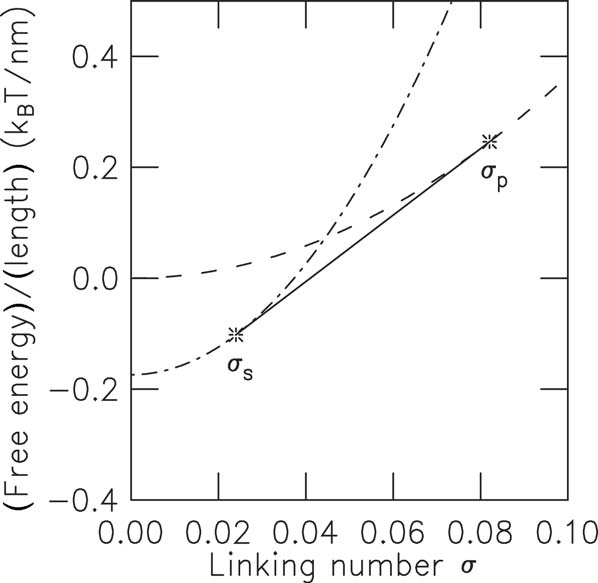
\includegraphics[width=.5\linewidth]{figures/marko_linking_number_graph}
    \caption{Plot of an example energy surface. Reproduced Figure 1 from \textcite{markoTorqueDynamicsLinking2007}.}
    \label{fig:marko_energy_surface}
\end{figure}
\subsubsection{Model formulation: internal melting}
Our model derives energy differences based on the difference between the (assumed to be locally linear) energy cost of increasing supercoiling in the exterior regions,
versus the integrated energy difference in the interior region. This means we model:
\[\Delta E = \tau(\sigma_0) \cdot 1.2 \cdot 2\pi + \int_{\sigma_0}^{\sigma_0 + \Delta \sigma_\text{RNAP}} \Delta z_\text{RNAP} \frac{\partial S}{\partial \sigma} d\sigma\]
for \(\Delta z_\text{RNAP} = 13 \text{bp} = 4.42 \text{nm}\) and \(\Delta \sigma_\text{RNAP} = -0.92\) as in \autoref{eq:delta_sigma_rnap}.

Given the well-defined structure of the RNAP-DNA complex and the fact that under all realistic physiological conditions \(\Delta \sigma_\text{RNAP} \gg \sigma_0\), we assume that the end-state energy is a constant, but unknown \(S_\text{unwound}\):
\begin{equation}
    \Delta E = \tau(\sigma_0) \cdot 1.2 \cdot 2\pi + \Delta z_\text{RNAP} \left(S_\text{unwound} - S(\omega_0)\right)
\end{equation}


However, when we compare the strength of this internal melting energy term to the ``exterior'' supercoiling term, we see that the external term dominates (\autoref{fig:app:energy_comparison}).
\begin{figure}[h]
    \centering
    %\includegraphics[width=.5\linewidth]{figures/energy_plot}
    \caption{Plotted is the binding energy required to bind an RNAP, for different starting values of \(\sigma_0\). In the single-phase regions, differences in \(\Delta E\) are dominated by the external torque term. In the two-phase region, \(\Delta E\) remains mostly constant!}
    \label{fig:app:energy_comparison}
\end{figure}
which means we can use the simple form:
\begin{equation}
    \Delta E = \tau(\sigma_0) \cdot 1.2 \cdot 2\pi
\end{equation}


\FloatBarrier
\subsubsection{Model evaluation}
This equation has some of the features that we wanted in the model. Consider the change in \(\Delta E\) by a \(\Delta \sigma\) change in the coexistence region where:
\[\tau = \frac{1}{\omega_0} \sqrt{2pg}{1 - \frac{p}{c_s}} = \text{constant}\]
\[S = \frac{-g}{1 - \frac{p}{c_s}} + \sqrt{\frac{2pg}{1 - \frac{p}{c_s}}} \sigma\]
for \(\sigma_2 = \sigma_1 + \Delta \sigma\). Then,
\[\Delta E_2 - \Delta E_1 = - \Delta z_\text{RNAP} \left( \frac{-g}{1 - \frac{p}{c_s}} + \sqrt{\frac{2pg}{1-\frac{p}{c_s}}} \Delta \sigma\right)\]

This means that we do not have a strictly constant binding energy in the constant-torque region. However, if we plot the value of \(\Delta E\) across various supercoiling values, for the mean value of constants given in \autoref{tab:constants}, we see that the unwinding energy does remain relatively constant in the constant torque regime!

The values for \(\Delta E\) are much larger than initially expected; Literature results show that the RNAP on-rate decreases roughly four-fold in the first single-phase region, which occurs for \(\Delta E \sim 4 \text{pN nm}\).

This discrepancy means that we expect our initial supercoiling-initiation model to be a useful way to upper-bound the effects of this behavior on the system. Realistically, secondary chromatin effects such as nucleosome displacement may allow for the high energy cost of adding polymerases to already supercoiled regions to be diminished.

\begin{figure}[h]
    \centering
    \begin{subfigure}{.49\linewidth}
        \centering
%        \includegraphics[width=.99\textwidth]{figures/time_plot}
        \caption{Plot of the inverse RNAP on-rate, as modeled here.}
    \end{subfigure}
    \begin{subfigure}{.49\linewidth}
        \centering
        %\includegraphics[width=.8\textwidth]{figures/revyakin_plot}
        \caption{Reproduced Figure 3c from \textcite{revyakinPromoterUnwindingPromoter2004}.}
    \end{subfigure}
    \caption{Our model predictions appear to replicate literature results. Even though \(\Delta E\) is not strictly constant in the two-phase/constant-torque region, its numerical value is nearly constant in that region.}
\end{figure}
\end{document}
